%! Author = louis
%! Date = 28-10-22

Le projet ayant comme contrainte principale d'etre disponible sur toutes les plateformes majeures une base web me parait évident.
Pourtant, le web vient aussi avec la limitation principale qu'est le besoin de connection permanente au serveur.\\\\
Pour remédier à ce problème une PWA ( Application Web Progressive ) nous permettrais de bénéficier des avantages du web,
tout en permettant aux utilisateurs de conserver une version locale de l'application.
De plus une PWA permet d'etre installée comme une application native Android ou IOS pour les plateformes mobiles ce qui facilite l'accès.\\

Une PWA comme toute application web nécessite plusieurs composant:
\begin{itemize}
    \item Une interface utilisateur
    \subitem un gestionnaire de données
    \subitem un gestionnaire de requêtes
    \subitem une libraire de composant graphique
    \item Une Couche de calcul applicatif et de persistance de donnée
    \subitem Une Base de Donnée
    \subitem Un ORM
    \subitem Une API définie
    \subitem Un système de matching pour le covoiturage
    \subitem Un système de création de trajet pour le covoiturage
    \subitem Un système de matching pour les dépenses
\end{itemize}
\subsubsection{TypeScript}
Avant de regarder quels outils utiliser pour les différents composants je pense qu'il est important de choisir un language de programmation.\\
Pour ce projet j'ai décidé d'utiliser le meme language pour les 2 composant majeurs que sont le front-end et le back-end.
Plusieurs choix s'offraient alors à moi, JavaScript, Kotlin, TypeScript ou n'importe quel langage compilable en web assembly\\
JavaScript n'était pas vraiment un bon choix vu qu'il ne propose pas de typage ce qui rend le code moin prédictible et robuste.\\
Kotlin est un bon candidat, il offre un typage statique, mais propose de l'inférence de type, peu être transpiler vers du JavaScript ou du web assembly,
les outils de développement pour kotlin sont aussi tres bon, mais la documentation pour une utilisation web est plutôt pauvre comparer aux autres options.\\\\
TypeScript a quant à lui tous les avantages de Kotlin, grace au typage fort, et profite aussi de la documentation et des outils javaScript grave à sa nature de superset.
Lorsque l'on développe un produit web surtout pour un développeur full-stack TypeScript est l'idéal.
Ces outils, l'environnement JavaScript, la sécurité des Types et du null, la documentation.
Pour toutes ces raisons TypeScript est le language idéal pour le développement Web.

\subsection{Front-end}\label{subsec:front-end}
Pour ce qui est de l'interface utilisateur ( le front end ) j'ai décidé d'utiliser Angular car ce framework utilise TypeScript nativement tout en supportent aussi les PWA
Angular étant un framework orienté m'oblige aussi à suivre une architecture propre qui permet de rendre independent les différents composants du projet .

\subsubsection{Gestion des données}
Pour conserver les données hors ligne et facilité l'accès a des données à jour lors d'une connexion j'ai decider d'utiliser NgRx.
Ce dernier est un framework de gestion de donnée qui simplifie l'accès et le caching de données
\subsubsection{Gestionnaire des requêtes}
Lorsque l'on veut interagir avec une API graphql il est preferable d'utiliser un client.\\\\
Il existe une multitude de clients GraphQl mais le plus populaire et le mieux documenter reste Apollo.
De plus il existe un wrapper pour le client Apollo qui l'intègre dans angular nommer Apollo Angular.
Je vais donc utiliser cette librairie pour récupérer mes données au pres de mon serveur .
\subsubsection{librairie CSS}
Utiliser une librairie de composant permet de simplifier la creation de l'interface grâce à des blocks de construction appeler composants\@.
Angular permet d'utiliser des librairies de composant avec leur propre logique, structure, et CSS\@.
Ces librairies fournissent aussi un ensemble de classe CSS pour rendre nos propres composants joli.\\
De plus elles permettent de rendre notre application responsive sans devoir y penser pour chaque composant.
Il existe plusieurs librairies majeures, les principales sont:
\begin{itemize}
    \item Angular Material
    \item PrimeNg
    \item NgBootstrap
\end{itemize}
Angular Material est la librairie officielle, elle est d'origine Google,
offre beaucoup de composant different en plus de plusieurs composants de layout qui permette de d'organiser d'autre composant sur la page.\\\\
PrimeNg offre aussi un grand nombre de composants, mais n'offre pas de layout par contre,
PrimeNg permet par contre d'utiliser un autre theme que Material.\\\\
NgBootstrap est un simple wrapper pour Bootstrap css et propose tous les composants de bootstrap.
Vu que mon objectif est de créer une PWA qui sera installable sur Android,
utiliser un theme similaire à ceux des applications Google intégrera mieux l'application.

\subsection{Back-end}\label{subsec:back-end}
Le serveur back-end doit être capable de mettre à disposition les données nécessaire au fonctionnement de l'application.
Cependant, le back-end sera aussi responsable des calculs d'équilibrage des dépenses, des matching de covoiturage et des trajets.\\\\
Connaissant deja Express.js et Spring ( Kotlin ) je me suis naturellement tourné vers ces derniers néanmoins je désirais utiliser du TypeScript pour ce projet.
Express.js est compatible avec TypeScript mais Spring ne l'est pas, Express.js est leger, minimaliste et propose une bonne documentation,
Spring est généraliste propose des outils de generation de code et utilise un système d'injection de dépendance.
Ce qu'il me fallait était une hybride entre Spring et Express.js.
Apres quelque recherche, j'ai trouvé un framework appeler Nest.js, ce dernier supporte nativement TypeScript, propose une documentation excellente,
propose un CLI permettant de générer du code boiler-plate, reste simple et leger, Utilise de l'injection de dépendance et est très utilisé et apprécié par d'autres développeurs.
J'ai donc décidé d'utiliser Nest.Js pour ce projet.

\subsubsection{ORM}
Nest.Js ( que je vais appeler Nest à partir de maintenant ) n'est pas un framework batteries included comme le sont Spring ou Laravel,
Il m'a alors fallu choisir aussi un ORM pour interfacer avec ma base de données.
Dans la Documentation de Nest, il y a des exemples de configuration avec les ORM les plus utilisés avec Nest et TypeScrip.
Ces derniers sont Sequelize, TypeOrm ainsi que Prisma,
ayant eu une experience avec Sequelize plutôt mauvaise lors de mon projet de dev3, j'ai décidé de regarder du côté de prisma.\\\\
Prisma est une ORM un peu particulière dans le sens où il propose d'utiliser un schema prisma pour définir ces entités au lieu d'utiliser du code TypeScript.
Cella me paraissait une très bonne chose vu que prisma générait alors lui-même les différents DTO nécessaires.
Il s'est cependant avéré qu'à l'utilisation prisma n'est pas l'idéale surtout lorsque l'on désire le coupler à une API graphQl.\\
À cause de son schema particulier, je devais définir le forma de mes entités à 2 endroits et tout de meme crée manuellement mes DTO\@.
Sans compter que les opérations de CRUD dans les entités était rendue tres complexe dû aux liens entre elles et que Prisma ne permet pas d'utiliser des identifiants.\\\\
J'ai donc décidé de jeter un œil à TypeOrm, celui-ci propose de définir les entités via des annotations TypeScript.
Ce qui me permet d'utiliser une seule classe pour définir mon entité d'ORM et de graphQl de plus TypeOrm est mieux
documenter grace au support d'une communauté plus large.


\subsubsection{L'API back end}
Il existe plusieurs types d'API tres utiliser pour le Back-end mais les plus populaires sont le REST et le SOAP\@.
SOAP est de moin en moin utiliser dû à la complexité intrinsèque du xml et à sa lourdeur.\\\\
Il nous reste alors REST qui est une bonne solution, mais nécessite pour presque chaque requête de récupérer des données qui ne seront pas toujours consommées par le client
Avec Rest l'on récupère une entité complete tous les champs sont renvoyés.
C'est pour cela que graphQl a ete crée, non seulement graphQL utilise un typage fort via un schema défini et exposer par le serveur,
mais en plus graphql permet de ne récupérer que les champs nécessaires au client grace au GQL .

\subsubsection{La base de donnée}
Ma base de donnée devais me permettre 2 chose, stocker des données géographique et faire des operation sur ces données.
Le seul choix qui s'offrait à moi compatible avec TypeOrm était Postgres avec une extension nommée POSTGIS\@.
Postgres est une base de donnée tres utiliser en production, est tres performante et stable.

\paragraph{Structure de donnée}
Pour stocker toutes les données nécessaires au fonctionnement de l'application, il nous faut une structure de donnée cohérente.
Voici un schema\ref{fig:dbSchema} de la base de donnée et de sa structure:
%Todo: fix possitioning Shema DB
\begin{figure}[h!]
    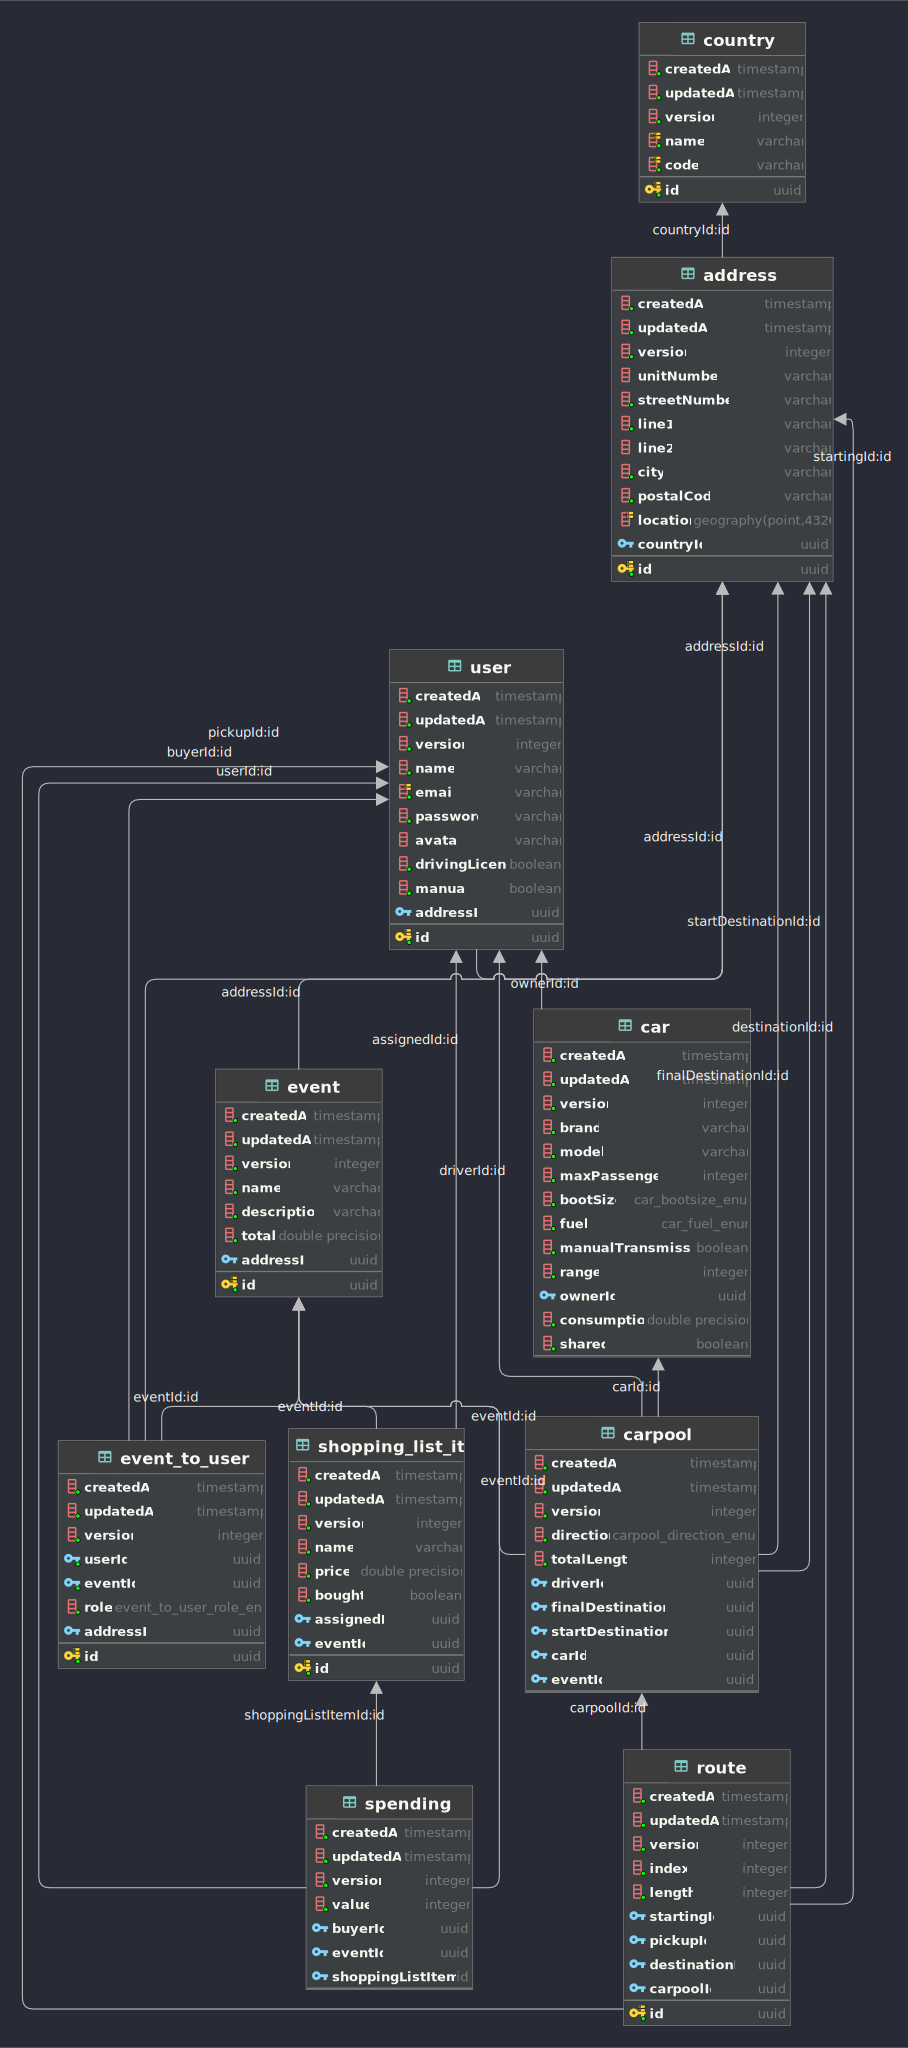
\includegraphics[width=\linewidth]{./images/dbShema}\caption{Architecture de la base de donnée}\label{fig:dbSchema}
    \centering
\end{figure}